\def\samplespace{(0,0) rectangle (1,1)}
\def\labelsamplespace{\draw (1,1) node[anchor=south] {$S$}}

\def\circlepartiala{(0.25,0.5) circle (0.2)}
\def\labelpartiala{\draw (0.25,0.7) node[anchor=south] {$A$}}
\def\circlepartialb{(0.6,0.4) circle (0.3)}
\def\labelpartialb{\draw (0.6,0.7) node[anchor=south] {$B$}}

\def\circleseparatea{(0.2,0.3) circle (0.1)}
\def\labelseparatea{\draw (0.23,0.25) node[anchor=north west] {$A$}}
\def\circleseparateb{(0.5,0.6) circle (0.2)}
\def\labelseparateb{\draw (0.5,0.8) node[anchor=south] {$B$}}

\def\circlefulla{(0.5,0.5) circle (0.35)}
\def\labelfulla{\draw (0.75,0.75) node[anchor=south west] {$A$}}
\def\circlefullb{(0.5,0.6) circle (0.15)}
\def\labelfullb{\draw (0.5,0.45) node[anchor=north] {$B$}}

\begin{center}
  \begin{tabular}{ccc}
    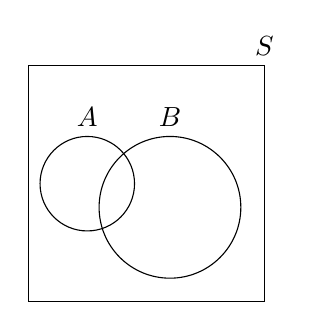
\begin{tikzpicture}
      \begin{scope}[scale=3]
        \draw \samplespace; \labelsamplespace;
        \draw \circlepartiala; \labelpartiala;
        \draw \circlepartialb; \labelpartialb;
      \end{scope}
    \end{tikzpicture}
    &
    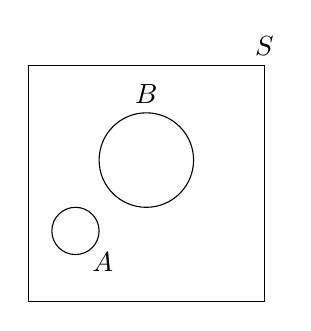
\begin{tikzpicture}
      \begin{scope}[scale=3]
        \draw \samplespace; \labelsamplespace;
        \draw \circleseparatea; \labelseparatea;
        \draw \circleseparateb; \labelseparateb;
      \end{scope}
    \end{tikzpicture}
    &
    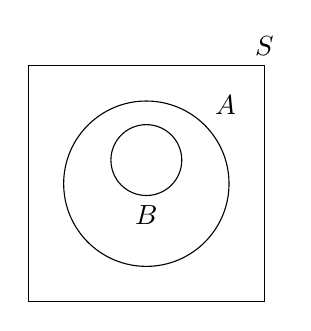
\begin{tikzpicture}
      \begin{scope}[scale=3]
        \draw \samplespace; \labelsamplespace;
        \draw \circlefulla; \labelfulla;
        \draw \circlefullb; \labelfullb;
      \end{scope}
    \end{tikzpicture}
    \\
    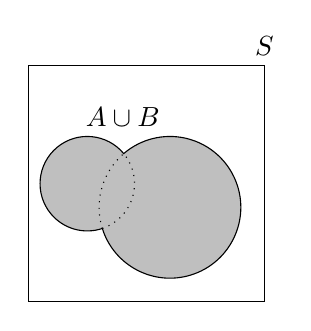
\begin{tikzpicture}
      \begin{scope}[scale=3]
        \draw \samplespace; \labelsamplespace;
        \draw[fill=lightgray] (0.31369, 0.31041) arc (-162.62:130.73:0.3cm) arc (39.54:288.57:0.2cm);
        \draw[dotted] (0.31369, 0.31041) arc (197.38:130.73:0.3cm) arc (39.54:-71.43:0.2cm);
        \draw (0.4,0.7) node[anchor=south] {$A \cup B$};
      \end{scope}
    \end{tikzpicture}
    &
    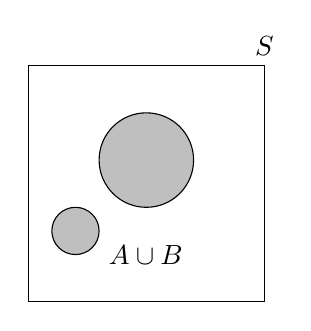
\begin{tikzpicture}
      \begin{scope}[scale=3]
        \draw \samplespace; \labelsamplespace;
        \draw[fill=lightgray] \circleseparatea;
        \draw[fill=lightgray] \circleseparateb;
        \draw (0.3,0.2) node[anchor=west] {$A \cup B$};
      \end{scope}
    \end{tikzpicture}
    &
    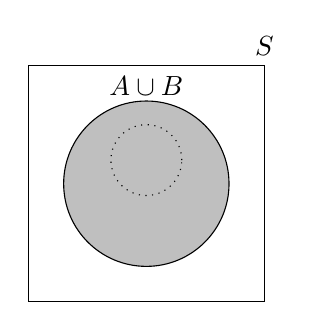
\begin{tikzpicture}
      \begin{scope}[scale=3]
        \draw \samplespace; \labelsamplespace;
        \draw[fill=lightgray] \circlefulla;
        \draw[dotted] \circlefullb;
        \draw (0.5,0.83) node[anchor=south] {$A \cup B$};
      \end{scope}
    \end{tikzpicture}
    \\
    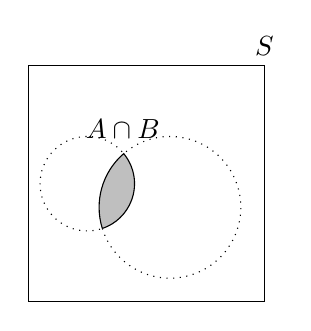
\begin{tikzpicture}
      \begin{scope}[scale=3]
        \draw \samplespace; \labelsamplespace;
        \draw[dotted] (0.31369, 0.31041) arc (-162.62:130.73:0.3cm) arc (39.54:288.57:0.2cm);
        \draw[fill=lightgray] (0.31369, 0.31041) arc (197.38:130.73:0.3cm) arc (39.54:-71.43:0.2cm);
        \draw (0.4,0.65) node[anchor=south] {$A \cap B$};
      \end{scope}
    \end{tikzpicture}
    &
    \begin{tikzpicture}
      \begin{scope}[scale=3]
        \draw \samplespace; \labelsamplespace;
        \draw[dotted] \circleseparatea;
        \draw[dotted] \circleseparateb;
      \end{scope}
    \end{tikzpicture}
    &
    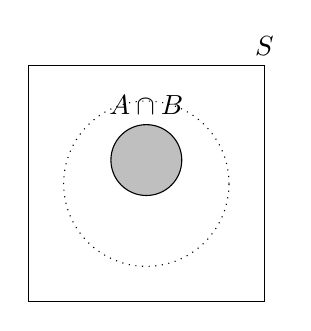
\begin{tikzpicture}
      \begin{scope}[scale=3]
        \draw \samplespace; \labelsamplespace;
        \draw[dotted] \circlefulla;
        \draw[fill=lightgray] \circlefullb;
        \draw (0.5,0.75) node[anchor=south] {$A \cap B$};
      \end{scope}
    \end{tikzpicture}
    \\
  \end{tabular}
\end{center}
